\documentclass[conference]{IEEEtran}
\IEEEoverridecommandlockouts
\usepackage{cite}
\usepackage{amsmath,amssymb}
\usepackage{graphicx}
\usepackage{booktabs}
\usepackage{url}
\usepackage{textcomp}
\def\BibTeX{{\rm B\kern-.05em{\sc i\kern-.025em b}\kern-.08em T\kern-.1667em\lower.7ex\hbox{E}\kern-.125em X}}

\begin{document}

\title{Collaborative Filtering for Movie Recommendation: A Comparative Study of Neighbourhood and Latent-Factor Methods on MovieLens}

\author{\IEEEauthorblockN{Manan, Dhanvi, Manav, and Krati}
\IEEEauthorblockA{Karnavati University, Ahmedabad, India\\
Machine Learning Course Mini-Project}}

\maketitle

\begin{abstract}
Recommender systems help users find relevant items in catalogues too large to browse. This paper builds and evaluates collaborative-filtering (CF) movie recommenders on the MovieLens \texttt{ml-latest-small} dataset (100,836 ratings, 610 users, 9,742 movies; 98.3\% sparse). We implement item-based and user-based $k$-nearest-neighbour CF with residual cosine similarity and shrinkage, and a biased matrix-factorisation (SVD) model, and compare them with global-mean, popularity and bias baselines. Hyper-parameters are tuned on a validation set carved out of the training data only, and final results are averaged over three random per-user 80/20 splits. Item-based CF gives the lowest rating-prediction error (RMSE $0.854\pm0.007$, against $0.876$ for the bias baseline and $1.045$ for the global mean) and the best top-10 ranking quality (NDCG@10 $0.245$, against $0.155$ for a popularity ranker). An ablation shows that ranking by predicted rating is a poor top-$N$ strategy (NDCG@10 $0.022$ for the same item-based model), whereas a similarity-sum score is effective: accuracy in rating prediction and quality of ranking are different objectives. We also provide an interactive demo application. All code is reproducible from fixed random seeds.
\end{abstract}

\begin{IEEEkeywords}
recommender systems, collaborative filtering, k-nearest neighbours, matrix factorisation, MovieLens, top-N recommendation
\end{IEEEkeywords}

\section{Introduction}
Online services offer far more movies than any viewer can inspect, so recommender systems are used to surface titles a particular user is likely to enjoy. \emph{Collaborative filtering} (CF) is the dominant approach: it uses only the pattern of past user--item ratings, on the premise that users who agreed in the past will agree in the future, and requires no item content~\cite{resnick1994,aggarwal2016}.

This mini-project studies CF on a public benchmark and answers three practical questions: (i) how much do personalised CF models improve over simple non-personalised baselines; (ii) how do neighbourhood methods compare with a latent-factor model; and (iii) does a model that predicts ratings well also produce good top-$N$ recommendation lists? Our contributions are:
\begin{itemize}
\item a complete, reproducible pipeline (preprocessing, leakage-free splitting, tuning, evaluation) implemented from scratch in Python with NumPy/SciPy;
\item a fair comparison of seven methods (four baselines and three CF models) on two tasks, rating prediction and top-10 ranking, with results averaged over three splits;
\item an ablation showing that the \emph{scoring rule} matters more than the choice of model for top-$N$ quality; and
\item an interactive web demo that serves recommendations for existing users, similar-movie lookup, and recommendations for a new user from a handful of ratings.
\end{itemize}

\section{Background and Related Work}
GroupLens introduced automated CF for netnews~\cite{resnick1994}. Item-based CF, which compares items rather than users, was shown to be accurate and scalable by Sarwar \emph{et al.}~\cite{sarwar2001} and underlies large-scale deployments~\cite{linden2003}; Deshpande and Karypis adapted it to top-$N$ recommendation by summing similarities to the items a user already likes~\cite{deshpande2004}. Latent-factor models such as matrix factorisation gained prominence for rating prediction~\cite{koren2009}, and Koren combined bias (baseline) predictors with neighbourhood and latent-factor information~\cite{koren2008}. Evaluation practice for CF, including the distinction between prediction accuracy and ranking metrics, is surveyed by Herlocker \emph{et al.}~\cite{herlocker2004}; McNee \emph{et al.} argue that accuracy metrics alone can mislead~\cite{mcnee2006}. We use the normalised discounted cumulative gain (NDCG) of J{\"a}rvelin and Kek{\"a}l{\"a}inen~\cite{jarvelin2002} for ranking quality.

\section{Dataset}
We use the MovieLens \texttt{ml-latest-small} release from GroupLens~\cite{harper2015}. It contains 100,836 star ratings (0.5--5.0 in half-star steps) by 610 users on 9,724 distinct movies (the movie table lists 9,742 titles); every user has at least 20 ratings. The target variable is the \texttt{rating} field. The user--movie matrix is 98.3\% empty; the median user has rated 70.5 movies, but the median movie has only 3 ratings and 66.4\% of movies have five or fewer (Fig.~\ref{fig:eda}), which makes the long tail hard for any CF method. The mean rating is 3.50. As the GroupLens documentation notes, this release is a \emph{development} dataset that may change over time and is not intended for shared research benchmarks; our numbers should therefore be read as a controlled comparison of methods on one fixed snapshot rather than as benchmark results.

\begin{figure*}[t]
\centering
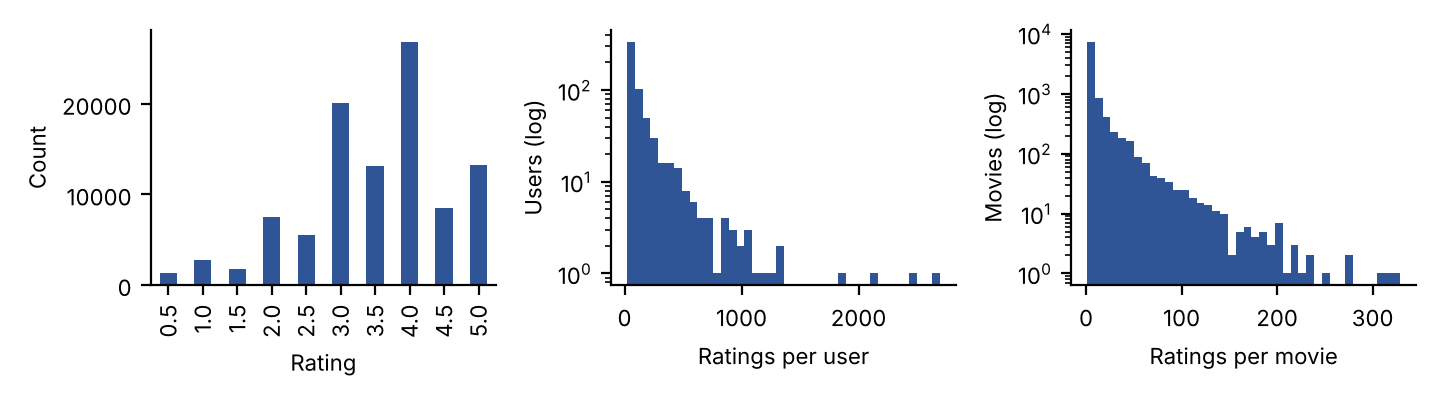
\includegraphics[width=0.95\textwidth]{eda.png}
\caption{Left to right: distribution of ratings; ratings per user; ratings per movie (log-scaled counts). Rating data are skewed towards 3--4 stars and heavily long-tailed across movies.}
\label{fig:eda}
\end{figure*}

\subsection{Preprocessing and data splitting}
We verified that the ratings file has no missing values and no duplicate (user, movie) pairs. User and movie identifiers are mapped to dense indices and the ratings are stored as a $610\times 9{,}724$ matrix $R$ with zeros for unobserved entries. No feature scaling is needed because models operate on rating residuals (Section~\ref{sec:models}).

To mimic predicting unseen ratings for known users, we hold out 20\% of \emph{each user's} ratings as the test set (at least one per user), so every user keeps training data. Hyper-parameters are tuned on a validation set formed by holding out a further 10\% of each user's \emph{training} ratings (seed 42 split); the test set is never used for tuning. After tuning, every model is refit on the full 80\% training portion and evaluated once on the test set. This is repeated for three random split seeds (42, 1, 2) and we report mean and standard deviation. All similarity statistics, biases and popularity counts are computed from training ratings only, which prevents leakage.

\section{Methodology}
\label{sec:models}
Let $r_{ui}$ be the rating of user $u$ for item $i$, $U_i$ the users who rated $i$, and $I_u$ the items rated by $u$.

\subsection{Baselines}
\textbf{Global mean:} predicts $\mu$ (the training mean) for every pair. \textbf{Popularity:} two non-personalised rankers: items ordered by number of training ratings, and by a damped mean rating. \textbf{Bias baseline:} $b_{ui}=\mu+b_u+b_i$ with regularised biases
\begin{equation}
b_i=\frac{\sum_{u\in U_i}(r_{ui}-\mu)}{\lambda_i+|U_i|},\quad
b_u=\frac{\sum_{i\in I_u}(r_{ui}-\mu-b_i)}{\lambda_u+|I_u|},
\end{equation}
with $\lambda_i=10$ and $\lambda_u=15$.

\subsection{Item-based $k$-NN collaborative filtering}
For each rated pair define the residual $\tilde r_{ui}=r_{ui}-b_{ui}$ (zero if unrated). The similarity between items $i$ and $j$ is the cosine of their residual vectors, shrunk towards zero when few users rated both:
\begin{equation}
s_{ij}=\frac{\sum_{u}\tilde r_{ui}\tilde r_{uj}}{\lVert\tilde r_{i}\rVert\,\lVert\tilde r_{j}\rVert}\cdot\frac{n_{ij}}{n_{ij}+\lambda_s},
\end{equation}
where $n_{ij}$ is the number of users who rated both. Each item keeps its $k$ most similar items $N_k(i)$. The predicted rating is
\begin{equation}
\hat r_{ui}=b_{ui}+\frac{\sum_{j\in N_k(i)\cap I_u}s_{ij}\,\tilde r_{uj}}{\delta+\sum_{j\in N_k(i)\cap I_u}|s_{ij}|},
\end{equation}
clipped to $[0.5,5]$, with damping $\delta\ge 0$. Neighbour lists are selected over the whole catalogue and then restricted at prediction time to items the user rated, a common efficient approximation.

\textbf{Ranking score.} Because predicted ratings ignore how much evidence supports them, we rank with the similarity-sum score of~\cite{deshpande2004},
\begin{equation}
\rho(u,i)=\sum_{j\in N_{k'}(i)\cap L_u}s_{ij},\qquad L_u=\{j:r_{uj}\ge 4\},
\end{equation}
with its own neighbourhood size $k'$.

\subsection{User-based $k$-NN}
The same construction is applied to users: $s_{uv}$ is the shrunk cosine of residual rows, the $k$ most similar users to $u$ are kept, and $\hat r_{ui}=b_{ui}+\sum_{v}s_{uv}\tilde r_{vi}/(\delta+\sum_{v}|s_{uv}|)$ over neighbours who rated $i$. Ranking uses the similarity-weighted sum of neighbours' ``liked'' indicators.

\subsection{Matrix factorisation (SVD)}
The latent-factor model predicts $\hat r_{ui}=\mu+b_u+b_i+\mathbf p_u^{\top}\mathbf q_i$ with $f$ factors, trained by stochastic gradient descent (learning rate 0.01, 20 epochs, factors initialised from $\mathcal N(0,0.1^2)$) on the regularised squared error $\sum(r_{ui}-\hat r_{ui})^2+\lambda(b_u^2+b_i^2+\lVert\mathbf p_u\rVert^2+\lVert\mathbf q_i\rVert^2)$~\cite{koren2009}. Top-$N$ lists rank by $\hat r_{ui}$.

\subsection{Hyper-parameter selection}
Rating hyper-parameters were chosen by validation RMSE over shrinkage $\lambda_s\in\{10,25,50,100\}$, $k\in\{40,\dots,640\}$ and $\delta\in\{0,2,5\}$ for item-based CF; $k\in\{10,\dots,320\}$ and $\delta\in\{0,2,5\}$ for user-based CF ($\lambda_s{=}10$); and $(f,\lambda)\in\{(20,0.05),(30,0.1),(60,0.1)\}$ for SVD. The ranking neighbourhood $k'$ was chosen by validation NDCG@10 over $\{20,\dots,400\}$ (item) and $\{10,\dots,160\}$ (user). Table~\ref{tab:hyper} lists the selected values.

\begin{table}[t]
\centering
\caption{Selected hyper-parameters.}
\label{tab:hyper}
\footnotesize
\begin{tabular}{lcccc}
\toprule
Model & $k$ & $\lambda_s$ & $\delta$ & $k'$ \\
\midrule
Item-based KNN & 640 & 100 & 0 & 20 \\
User-based KNN & 320 & 10 & 2 & 40 \\
SVD & \multicolumn{4}{c}{$f=60$, $\lambda=0.1$, 20 epochs} \\
\bottomrule
\end{tabular}
\end{table}

\section{Evaluation Protocol}
\textbf{Rating prediction} is measured by RMSE and MAE on all held-out ratings. \textbf{Top-$N$ recommendation} is evaluated per user by ranking every movie the user has not rated in training and taking the top $K=10$; a recommended movie is \emph{relevant} if the user rated it $\ge 4$ in the test set. We report Precision@10, Recall@10, Hit Rate@10 (fraction of users with at least one relevant item in their list), and NDCG@10 with binary gains, $\mathrm{NDCG@}K=\mathrm{DCG@}K/\mathrm{IDCG@}K$. Only users with at least one relevant test item are scored (597--601 of 610 users depending on the split). Catalogue coverage is the share of movies that appear in at least one user's list. Because popularity-count and ranking scores are not rating-valued, RMSE/MAE are not reported for the count-based popularity ranker, and the global mean (a constant) is not ranked.

\section{Results}
\subsection{Main comparison}
Table~\ref{tab:main} and Fig.~\ref{fig:comp} summarise the results. For rating prediction, every personalised model beats the global mean (RMSE 1.045) and the popularity mean (0.977). The bias baseline already reaches 0.876; item-based CF improves on it to $0.854$, and user-based CF and SVD reach about $0.864$. The gaps between the personalised models are small (about 0.01 RMSE), but item-based CF was better than both user-based CF and SVD in each of the three splits (by 0.0095--0.0115 RMSE), and better than the bias baseline by 0.021--0.022 in every split.

For top-10 ranking, item-based CF with the similarity-sum score is clearly best: NDCG@10 $0.245$ versus $0.155$ for ranking by popularity count, $0.145$ for user-based CF and $0.102$ for the bias baseline, and at least one relevant movie appears in the top-10 list of $70.6\%$ of users (popularity: $55.3\%$). Item-based CF also recommends a broader part of the catalogue than popularity (coverage 5.2\% vs.\ 0.5\%), although user-based CF covers more (10.3\%). SVD, ranked by predicted rating, performs poorly on this task (NDCG@10 $0.018$), despite its competitive RMSE.

\begin{table*}[t]
\centering
\caption{Test-set results (mean\,$\pm$\,std over three random 80/20 per-user splits). Rating metrics: lower is better. Ranking metrics at $K{=}10$ (relevant = held-out rating $\geq 4$): higher is better. Best per column in bold.}
\label{tab:main}
\small
\begin{tabular}{lcccccc}
\toprule
Model & RMSE & MAE & P@10 & R@10 & NDCG@10 & HR@10 \\
\midrule
Global mean & 1.045\,$\pm$\,0.003 & 0.829\,$\pm$\,0.002 & -- & -- & -- & -- \\
Popularity (rating count) & -- & -- & 0.117\,$\pm$\,0.003 & 0.096\,$\pm$\,0.004 & 0.155\,$\pm$\,0.007 & 0.553\,$\pm$\,0.012 \\
Popularity (damped mean) & 0.977\,$\pm$\,0.006 & 0.763\,$\pm$\,0.003 & 0.098\,$\pm$\,0.002 & 0.075\,$\pm$\,0.003 & 0.122\,$\pm$\,0.003 & 0.487\,$\pm$\,0.010 \\
Bias baseline & 0.876\,$\pm$\,0.007 & 0.676\,$\pm$\,0.004 & 0.080\,$\pm$\,0.005 & 0.058\,$\pm$\,0.004 & 0.102\,$\pm$\,0.004 & 0.423\,$\pm$\,0.008 \\
User-based KNN & 0.864\,$\pm$\,0.007 & 0.665\,$\pm$\,0.004 & 0.111\,$\pm$\,0.001 & 0.097\,$\pm$\,0.001 & 0.145\,$\pm$\,0.002 & 0.538\,$\pm$\,0.016 \\
Item-based KNN & \textbf{0.854\,$\pm$\,0.007} & \textbf{0.653\,$\pm$\,0.004} & \textbf{0.182\,$\pm$\,0.002} & \textbf{0.154\,$\pm$\,0.003} & \textbf{0.245\,$\pm$\,0.004} & \textbf{0.706\,$\pm$\,0.010} \\
SVD (matrix factorisation) & 0.864\,$\pm$\,0.007 & 0.664\,$\pm$\,0.004 & 0.016\,$\pm$\,0.006 & 0.012\,$\pm$\,0.005 & 0.018\,$\pm$\,0.009 & 0.131\,$\pm$\,0.046 \\
\bottomrule
\end{tabular}
\end{table*}

\begin{table}[t]
\centering
\caption{Effect of the ranking score and of a minimum-support filter (candidates with $\geq 20$ training ratings). Mean over three splits.}
\label{tab:ablation}
\footnotesize
\setlength{\tabcolsep}{3pt}
\begin{tabular}{lccc}
\toprule
Variant & P@10 & NDCG@10 & HR@10 \\
\midrule
Item-KNN / similarity-sum score & 0.182 & 0.245 & 0.706 \\
Item-KNN / similarity-sum score + support filter & 0.182 & 0.244 & 0.704 \\
Item-KNN / predicted-rating score & 0.022 & 0.022 & 0.108 \\
Item-KNN / predicted-rating score + support filter & 0.078 & 0.090 & 0.384 \\
SVD / predicted-rating score & 0.016 & 0.018 & 0.131 \\
SVD / predicted-rating score + support filter & 0.039 & 0.045 & 0.256 \\
\bottomrule
\end{tabular}
\end{table}


\begin{figure*}[t]
\centering
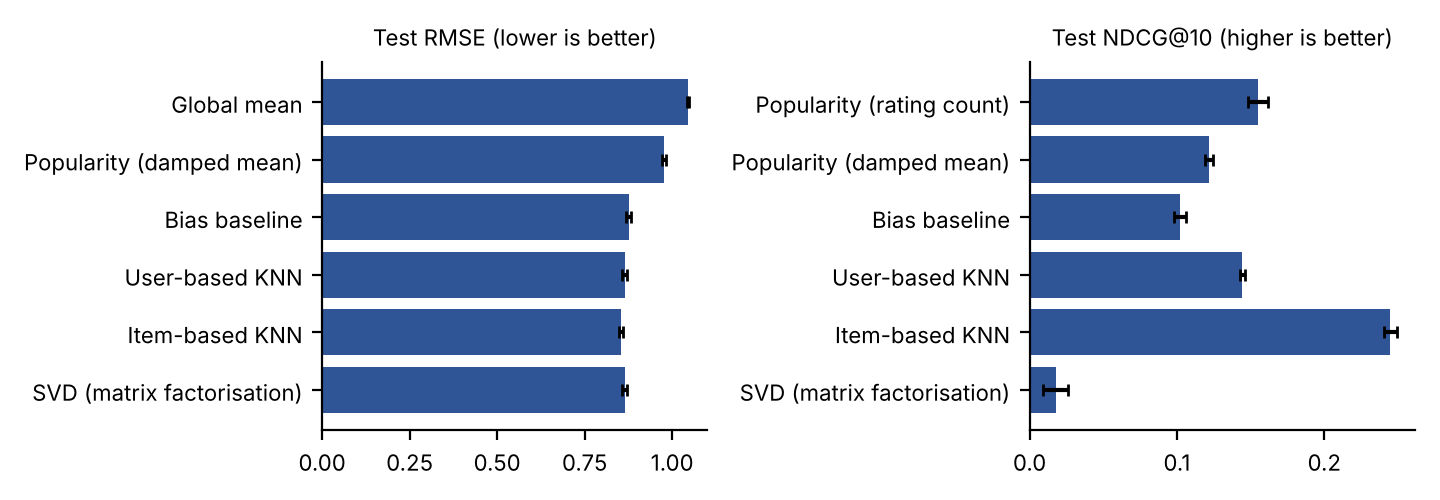
\includegraphics[width=0.85\textwidth]{comparison.png}
\caption{Test RMSE (left) and NDCG@10 (right) for each model; bars show means and error bars one standard deviation over three splits.}
\label{fig:comp}
\end{figure*}

\subsection{Why does ranking quality differ from rating accuracy?}
Table~\ref{tab:ablation} isolates the scoring rule. Ranking the item-based model's candidates by predicted rating drops NDCG@10 from $0.245$ to $0.022$. A likely explanation is that a predicted rating can be extreme for a movie supported by only one or two neighbours, so such movies crowd the list although few users have actually enjoyed them; a similarity-sum score instead rewards movies that are strongly related to many of the user's liked movies. Restricting candidates to movies with at least 20 training ratings recovers part of the loss (NDCG@10 $0.090$ for item-based and $0.045$ for SVD) but does not close the gap, so the scoring rule is the main factor. This agrees with the general observation that accuracy metrics do not necessarily predict recommendation quality~\cite{mcnee2006,herlocker2004}. SVD would likely rank better with a ranking-oriented loss or a popularity-aware score, which we did not tune.

\subsection{Sensitivity to neighbourhood size}
Fig.~\ref{fig:k} shows validation behaviour. RMSE for item-based CF improves steadily as $k$ grows, and shrinkage helps modestly, with little difference between $\lambda_s=50$ and $100$ (the selected values lie at the edge of our grid, so larger values might help). Ranking quality, in contrast, is nearly flat for $k'\ge 50$ and best at the smallest value tried ($k'=20$), consistent with the intuition that only the strongest neighbours matter for ranking.

\begin{figure*}[t]
\centering
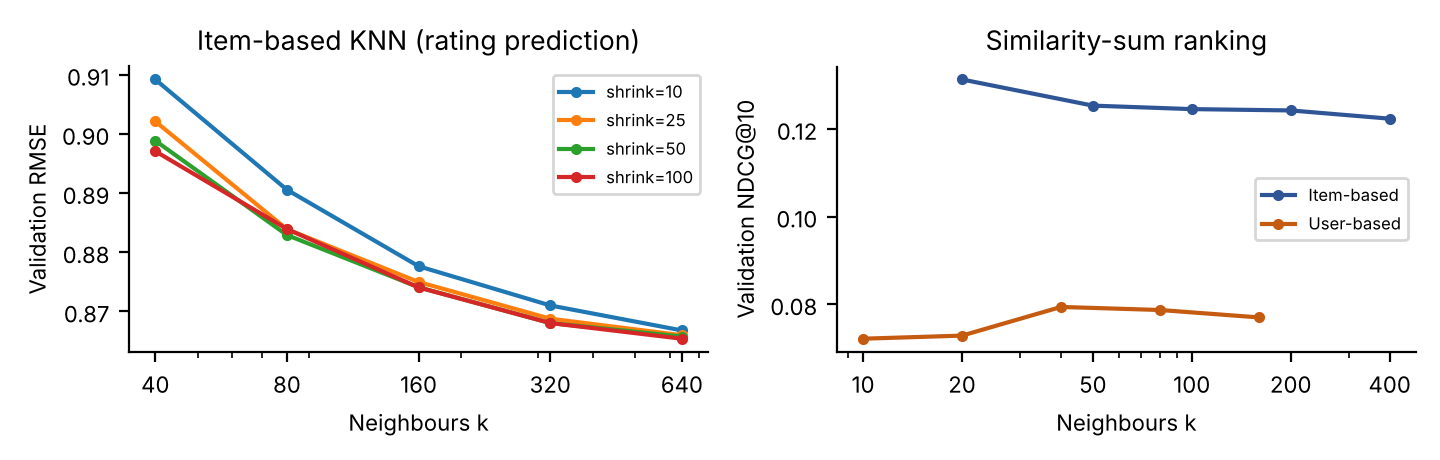
\includegraphics[width=0.85\textwidth]{k_sensitivity.png}
\caption{Validation results. Left: item-based RMSE versus $k$ for several shrinkage values (best damping). Right: validation NDCG@10 of the similarity-sum score versus neighbourhood size.}
\label{fig:k}
\end{figure*}

\subsection{Qualitative examples}
Using the deployment model trained on all ratings, the five movies most similar to \emph{Toy Story (1995)} are \emph{Aladdin (1992)} (0.145), \emph{Toy Story 2 (1999)} (0.143), \emph{Back to the Future (1985)} (0.099), \emph{Finding Nemo (2003)} (0.097) and \emph{The Incredibles (2004)} (0.093): sequels and family animation or adventure films, as expected. For user~1, whose highest-rated movies include \emph{Seven (1995)}, \emph{The Usual Suspects (1995)} and \emph{X-Men (2000)}, the top recommendations are \emph{Terminator~2: Judgment Day}, \emph{Aliens}, \emph{The Godfather}, \emph{Die Hard} and \emph{The Shawshank Redemption}. These examples are illustrative, not evidence of accuracy.

\section{Demonstration Application}
The deployment model (item-based CF trained on all 100,836 ratings) is served by a Streamlit application with three views: recommendations for an existing user with the user's top-rated movies for context; a ``movies like \ldots'' lookup based on item similarity; and a new-user mode in which a visitor rates a few movies and immediately receives recommendations. Because the item-based model only needs the new user's ratings and the stored neighbour lists, no retraining is required for new users. A filter hides movies with very few ratings.

\section{Limitations and Future Work}
Results come from one small dataset with a random per-user hold-out rather than a chronological split, which can be optimistic relative to real deployment. The three-split standard deviations quantify split variability but not tuning variability, and no formal significance test was run. Some selected hyper-parameters lie at the edge of the search grid, SVD was tuned over only three configurations, and a ranking-oriented factorisation model (e.g.\ with pairwise loss) was not tried, so the comparison with SVD should not be read as a general verdict on matrix factorisation. The evaluation is offline and treats unobserved movies as non-relevant, which understates true precision; we did not run a user study. The models cannot recommend for users or movies with no ratings (cold start). Future work includes a hybrid model that adds content features such as genres and external movie metadata, temporal evaluation, implicit-feedback and pairwise-ranking methods, and diversity and novelty metrics.

\section{Conclusion}
On MovieLens \texttt{ml-latest-small}, item-based collaborative filtering with residual cosine similarity and shrinkage was the best of the compared models for both rating prediction (RMSE $0.854$) and top-10 ranking (NDCG@10 $0.245$), consistently across three random splits. The gains in RMSE over simple baselines are modest, whereas the choice of ranking score changes top-$N$ quality by an order of magnitude. Practitioners should therefore evaluate recommenders on the task they will actually perform and not rely on rating error alone.

\section*{Reproducibility}
Code, data-loading instructions and the demo application are provided with this paper. Running \texttt{python run\_experiments.py} reproduces every table and figure (seeds 42, 1, 2; NumPy~\cite{harris2020}) and \texttt{streamlit run app.py} starts the demo.

\bibliographystyle{IEEEtran}
\bibliography{references}

\end{document}
